\section{MobiScope Overview}
\label{sec:platform}

% This section describes the goals for our monitoring approach, and how
% \platname achieves these goals using proxying.  We show that our
% approach imposes reasonable overheads, and we describe how our
% IRB-approved study protects user privacy.

% \subsection{Goals}
% \label{sec:goals}
% Our primary goal is \emph{to monitor all the Internet traffic from
%   mobile devices regardless of the operating system, wireless access
%   technology, and the ISPs used by the mobile device}.  To achieve
% this goal, we identify the following desirable properties for a
% measurement platform:
% \begin{packedenumerate}
% \item \emph{Portable.} Our approach should work on all major device
%   OSes without requiring support from carriers or ISPs.
% \item \emph{Pervasive.} We should be able to measure traffic
%   regardless of the location, access technology, and ISPs used by
%   mobile devices.
% \item \emph{Passive.} We wish to understand the network traffic
%   naturally generated by users and their devices, requiring passive
%   monitoring.
% \item \emph{Deployable.} We want a low barrier to entry to facilitate
%   large-scale adoption with minimal impact on the user
%   experience. \tbd{We need to say easy to controlled perform
%     experiments}
% \end{packedenumerate}

In this section, we present an overview of the \platname{} platform\footnote{Our platform is currently in private beta with deployments in the US, France and China. We will make the \platname{} software publicly available.}. The goal of \platname{} is straightforward: we 
 seek to enable passive monitoring of \emph{all
  the Internet traffic from and to mobile devices}. While previous work has accomplished 
  this for a limited set of devices or networks, we seek to avoid such limitations: 
\begin{packedenumerate}
\item \emph{OS agnostic.} Monitor traffic independently of
  the OS run by the monitored device. In particular, we avoid the need to 
  develop OS-specific applications, or to root or jailbreak the phone.
\item \emph{ISP agnostic.} Monitor traffic without any
  support from ISPs and cellular providers.
\item \emph{Access technology agnostic.} Monitor traffic
  whatever the access technology used by the mobile device (Wifi, GSM,
  CDMA, UMTS, LTE, etc.)
\item \emph{Continuous.} Monitor traffic continuously, even when devices switch 
between networks or return from being idle.

%\item \emph{Flow modification.} We want to not only monitor, but
 % also possibly modify data packets in order to experiment. This makes
 % \platname{} both a passive monitoring and an experimental
 % platform. 
\item \emph{Scalability.} \platname{} should be equally feasible to deploy 
on a single machine or using a collection of VMs in a hosted/cloud deployment. 

\item \emph{Encryption agnostic.} Achieve visibility of both encrypted and plaintext traffic.

 \end{packedenumerate}    
 

In the following, we describe in detail the design of \platname{},
then we discuss the limitations of the platform.


\subsection{MobiScope Design}

% We now describe how we achieve these goals using proxying.
% Specifically, we use two approaches to proxy mobile traffic: secure
% proxying via virtual private networks (VPNs) and insecure transparent
% proxying.  These two approaches allow us to measure traffic with and
% without carrier interposition, respectively.

% \subsubsection{VPN Proxying}
% \label{sec:platform-vpn}

To meet the above goals, we exploit the observation that nearly all 
devices support network traffic indirection via virtual private networks (VPNs). 
In particular, instead of using the VPN server to access a private network, 
we use it as a proxy for all of a device's mobile Internet traffic. This enables passive monitoring 
of Internet traffic regardless of device OS, carrier/ISP or access technology. 
Further, we show that this approach has minimal impact on 
performance and measurement fidelity -- making \platname{} a practical 
approach for pervasive passive network monitoring.

In the following sections, we describe how our measurement infrastructure 
achieves the goals states in the previous section. We begin by describing 
how we addressed several challenges with implementing our VPN-based 
proxy. 


% designed the \platname{} platform
%on a VPN infrastructure. By instrumenting the VPN server that
%mobile devices are using, we can monitor all the Internet traffic going
%through the VPN tunnels. But, using a VPN infrastructure raises three
%important questions. i) How ubiquitous is the VPN technology on mobile
%devices?  ii) How to monitor traffic on \platname{}? iii) How to
%modify traffic on \platname? We explore in the following these three key questions.

\subsubsection{VPNs for Mobile Devices}
\label{sec:vpn-tech-mobile-device}
In this section, we provide a detailed description of how VPNs allow 
us to achieve many of our \platname{} design goals.  
Our first goal is to provide a measurement system that works regardless 
of device OS. To achieve this goal, we note that VPNs are widely supported 
on the most popular mobile OSes. Indeed, Android, BlackBerry, Bada, and iOS all support VPNs,
primarily to satisfy their enterprise clients. In this work, we focus on 
the two most popular OSes: iOS and Android. 

Our second and third goals are 
to enable measurements regardless of ISP or access technology. 
Fortunately, iOS and Android support VPN connectivity regardless of  
ISP or access technology -- so long as the network supports the Internet Protocol. 

We note that both iOS and Android support VPN connections 
using the IPSec standard, meaning we can implement our VPN proxy 
server using robust, open-source code from Strongswan~\cite{strongswan}. 
\platname{} thus supports IPSec tunnels using either IKEv1 or
IKEv2~\cite{rfc5996} for authentication and key negotiation.


To meet our goal of continuous network monitoring,
a VPN must always be enabled. Currently, all iOS devices (version 3.0
and above) support a feature called \textit{VPN On-Demand}.  VPN
On-Demand forces the iOS device to use VPN tunnels when connecting to
a specified set of domains. To ensure all possible addresses match this list, 
we observed that iOS uses suffix matching to determine which connections 
should be tunneled; accordingly, we specified the domain list as the set of 
alphanumeric characters (a-z, 0-9, one character per domain). 
Android version 4.2 and above support an
\textit{Always On VPN} connection that is always enabled for all data
traffic, and Android version 4.0 and above provide an API that allows
applications to manage VPN tunnels. We support both options: we have distributed Always On VPN 
configurations and implemented an application that
uses the VPN API to provide equivalent functionality for
Android 4.0 and 4.1.


% The use IPsec by mobile devices for pervasive VPN tunnels limited our
% choice of VPN daemons to manage VPN tunnels on our proxying server.
% Though VPN daemons manage tunnels created using protocols such as PPTP
% and L2TP, the ``VPN On-Demand'' feature of iOS is available only for
% VPN tunnels that use IPsec.  To the best of our knowledge, the only
% publicly available VPN daemon that uses IPsec in Linux \emph{without
%   any kernel modifications} is Strongswan~\cite{strongswan}.
% Strongswan also supports the faster IKEv2~\cite{rfc5996} based
% authentication which is supported by Android devices.

% \subsubsection{Advantages and Drawbacks of VPNs}
% \label{sec:advant-drawback-vpn}



\subsubsection{Monitoring Traffic on MobiScope}
\label{sec:monit-traff-mobiscope}



Having shown that VPNs support many of \platname{}'s goals, 
we now describe how we implement passive network monitoring 
using VPN proxying. While the high-level design for capturing 
network traffic from mobile devices is straightforward, the implementation 
is not. In particular, the interactions between IPSec, routing and NAT 
complicate our ability to map bidirectional flows to individual devices. 
The following paragraphs describe these challenges and how we 
addressed them to provide a stand-alone (\ie single server) mobile-traffic monitoring 
proxy. We conclude by describing how our architecture facilitates 
pluggable modules for performing custom monitoring.

At first glance, capturing all traffic traversing a VPN server should be 
as simple as running a tap on the network interface, \eg using \textit{tcpdump}. 
While this indeed captures all traffic, it does not capture sufficient information 
to distinguish bidirectional flows and map them to individual devices. We now 
describe how to provide this mapping.

First, we describe how the Linux network stack interacts with IPSec. 
We assume the \platname{} server is assigned 
IP address $m$ and the mobile device's public IP address is $d$. When 
the VPN connection is established, the proxy assigns the device a private address 
$v$. Last, the device is attempting to access a service located at address $w$. 
We denote a packet from source $s$ to destination $d$ as $s \rightarrow d$.

\noindent \textbf{Forward path.} The first step is to map flows in the forward direction. Figure~\ref{fig:packet-monitor-a} shows the path that packets take 
through a \platname{} proxy.  At steps (1),
(2), and (3) the encrypted datagram (in gray, $d \rightarrow m$) is passed to the IPSec 
module to decrypt and process the encapsulated IP datagram ($v \rightarrow w$) sent from 
the device. Because the \platname{} assigns private address space to 
clients, it must use NAT in step (5) to convertthe private IP address \emph{v} to the public IP
address \emph{m}. Last, the packet is forwarded to the Internet. 

We now describe how running tcpdump and tracking the NAT table are 
sufficient for mapping flows in the forward direction. Running \emph{tcpdump} on the Ethernet device captures packets at 
step (2), (4), and (7). The translation table provides a map between the public IP address \emph{d}
of the device and its private IP address \emph{v} in the tunnel. To
associate packets to a device and a Web service, we only need the
packet captured at step (4) that associates the packet to the private
address \emph{v} of the device in the VPN tunnel and the Web service
(address \emph{w}), and the translation table that gives the
mapping between the device in the VPN tunnel (address \emph{v}) and
the public IP address \emph{d} of the mobile device.

\noindent \textbf{Reverse path.} In the reverse direction (when packets flow from the
Internet to the mobile device), it is no longer possible to associate a
mobile device to the packets. We refer to 
Figure~\ref{fig:packet-monitor-b}, where we continue to dump packets from 
the Ethernet device. From
steps (2) and (7), we know that a packet in sent by the service at address $w$ to
the \platname{} box (step (2)), but then this packet is encapsulated
at the IPsec layer -- address resolution is performed by the NAT
without passing through tcpdump. So, when we see the datagram at step (7), we have no
way to know which encrypted packet is encapsulated. We need to dump
the packet at step (4), but we have no access to it via the standard Linux networking stack. 

\noindent \textbf{Bidirectional mappings.} A straightforward solution to 
the reverse path mapping problem is to forward traffic to a separate NAT 
device and dump traffic there. To avoid the need for additional hardware/VMs,
we simply virtualize an additional network interface and route traffic through it. 

Namely, we use a Linux TUN device, send packets from \emph{w} to \emph{v} through 
it and run packet captures on that TUN device (Figure~\ref{fig:packet-monitor-d}). 
Indeed, when a packet is
received from the Internet and arrives at NAT at step
(3), the NAT resolves the public address of the
\platname{} box \emph{m} to the address of the device in the VPN
tunnel \emph{v}. We design the NAT such that each client is assigned an 
address from a space of prefix length $p-1$. The $p$th bit has a
specific role. By default it is set to 0, but we modified the NAT so
that when it receives a packet that resolve to \emph{v}, it changes it
to \emph{v'} that only differ from \emph{v} by the $p$th bit that is
set to 1. This facilitates routing traffic to the TUN device for all
packets whose destination is \emph{v}, and facilitates forwarding  
all packet with a \emph{v'} destination address ($p$th bit set
to 1) to the TUN device, step (5). Then, we implement a process at the
TUN device that changes the destination address
from \emph{v'} to \emph{v}, and to sends the packet to the IP
layer, step (6). Then the packet follows the path of a regular packet
in a VPN tunnel. 

When a packet is received from the mobile device, we perform a similar
process that is described in Figure~\ref{fig:packet-monitor-c}. 

%In summary, exploiting the notion of TUN device, we are now able to
%dump all Internet traffic from and to a mobile device connected to the
%\platname{} platform from a single machine, and to associate this
%traffic to corresponding mobile devices and Web services. 

\begin{figure}
\begin{center}
  \subfloat[Packet from mobile device. \emph{Tcpdump can capture
    packets at step (2)~d~$\rightarrow$~m, (4)~v~$\rightarrow$~w, and
    (7)~m~$\rightarrow$~w.}]{\label{fig:packet-monitor-a}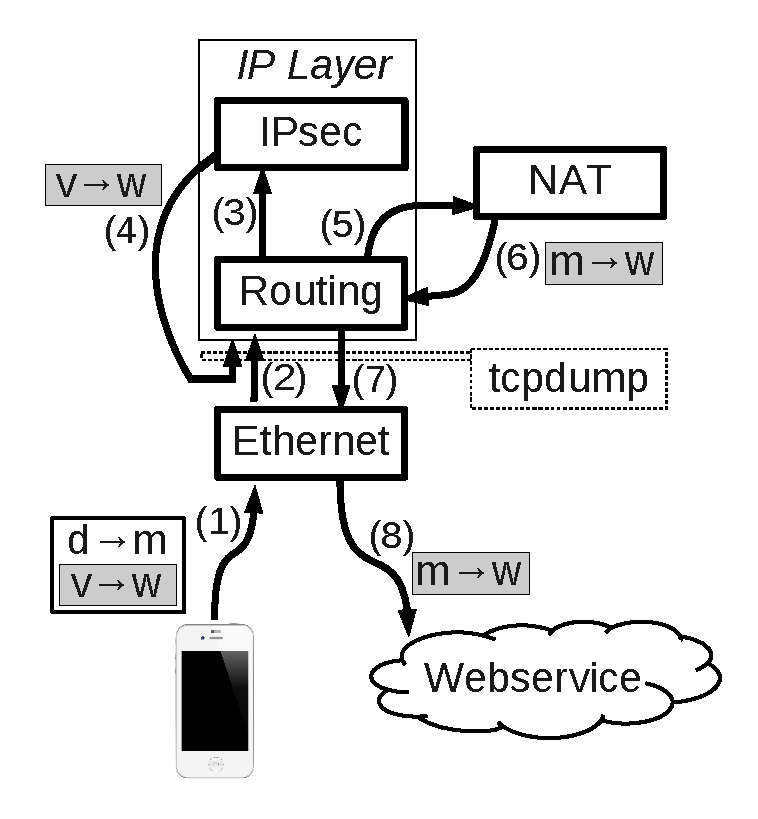
\includegraphics[width=0.47\columnwidth]{figures/packet-monitoring-a.pdf}}
  \hspace{0.05\columnwidth} \subfloat[Packet to mobile
  device. \emph{Tcpdump can capture packets at step
    (2)~w~$\rightarrow$~m and (7)~m~$\rightarrow$~d, however it is
    cannot log the packet
    w~$\rightarrow$~v.}]{\label{fig:packet-monitor-b}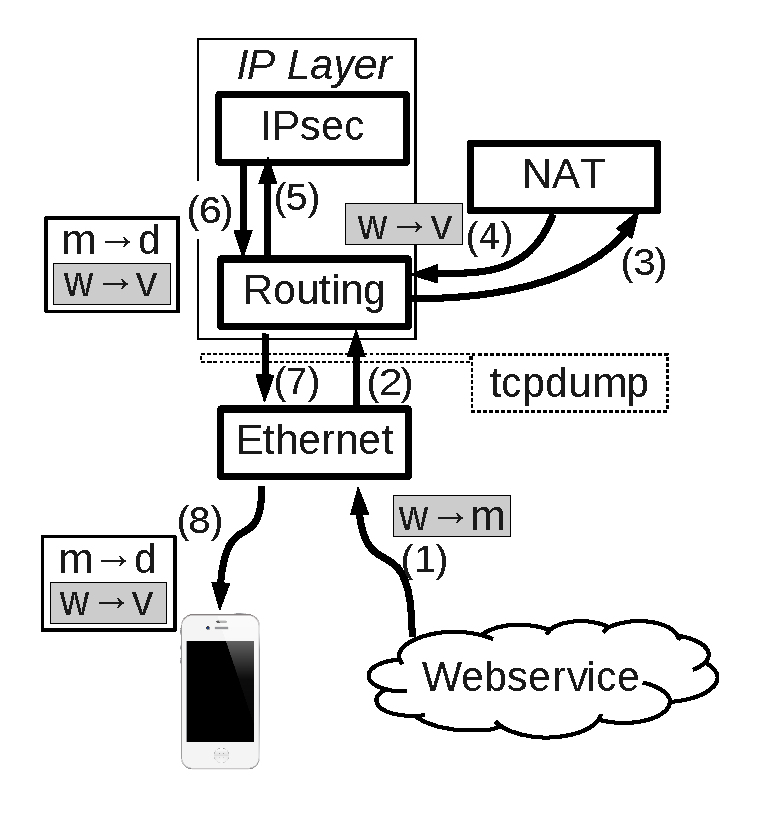
\includegraphics[width=0.47\columnwidth]{figures/packet-monitoring-b.pdf}}
  \newline \subfloat[Packet from mobile device. \emph{Tcpdump
    monitoring packets on the tun device can capture packets at step
    (5)~v~$\rightarrow$~w, and
    (6)~v'~$\rightarrow$~w.}]{\label{fig:packet-monitor-c}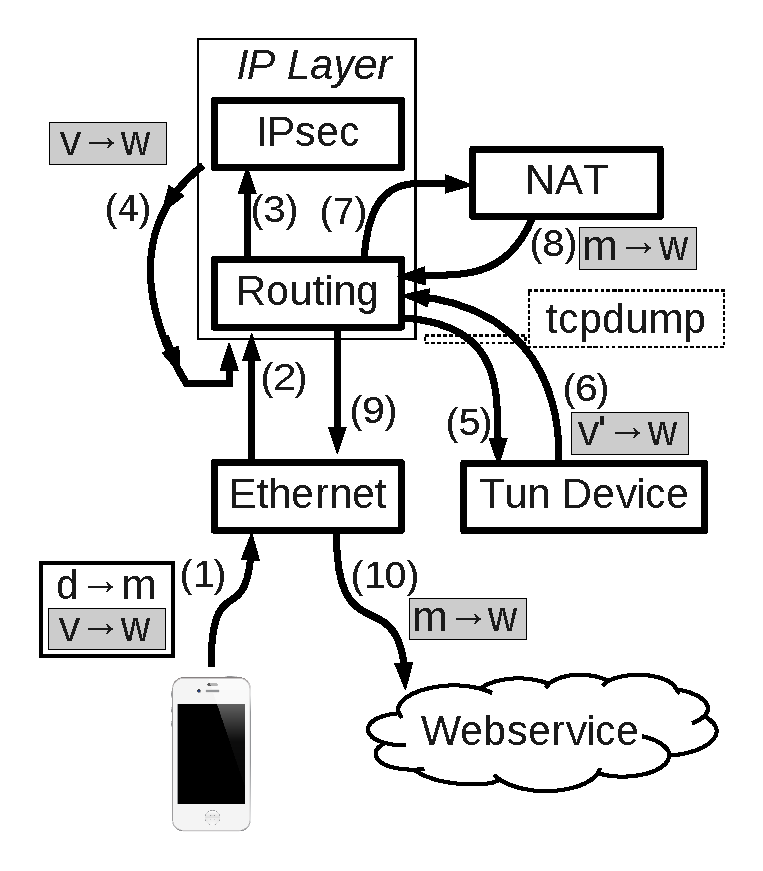
\includegraphics[width=0.47\columnwidth]{figures/packet-monitoring-c.pdf}}
  \hspace{0.05\columnwidth} \subfloat[Packet to mobile
  device. \emph{Tcpdump monitoring packets on the tun device can
    capture packets at step (5)~w~$\rightarrow$~v', and
    (6)~w~$\rightarrow$~v.}]{\label{fig:packet-monitor-d}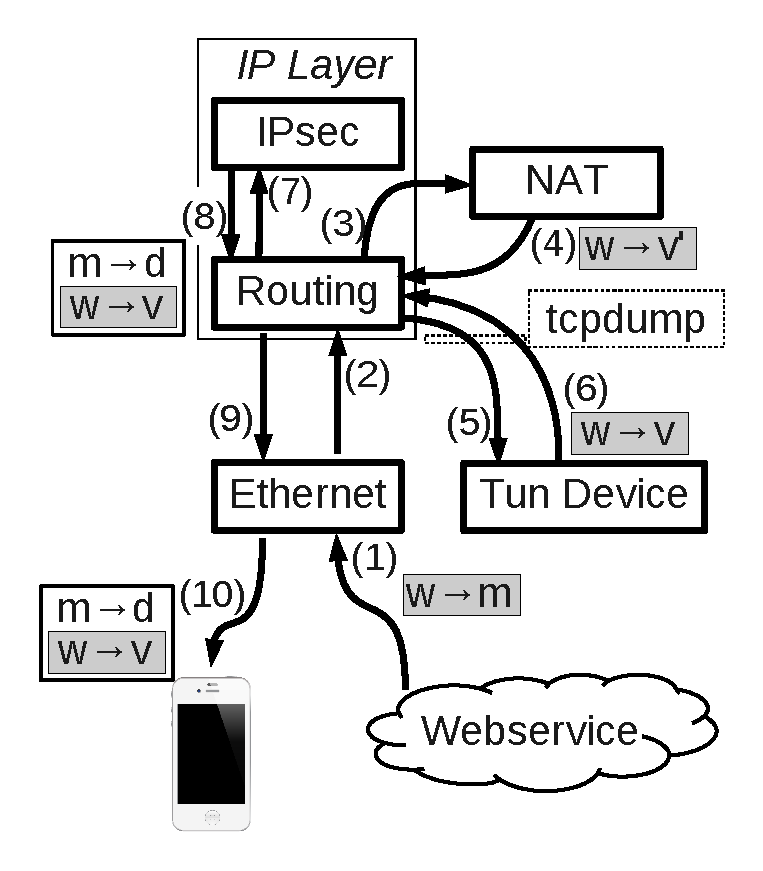
\includegraphics[width=0.47\columnwidth]{figures/packet-monitoring-d.pdf}}
  \newline
\begin{small}
\begin{tabular}{|c|p{0.8\columnwidth}|}
\hline
Symbol & Description \tabularnewline
\hline
d & IP address of the mobile device assigned by its ISP. \tabularnewline
m & IP address of the \platname server. \tabularnewline
w & IP address of the server providing the Web service. \tabularnewline
(i) & The i-th step of packet processing. \tabularnewline
\fbox{a $\rightarrow$ b} & Packet with source IP \emph{a} and destination IP \emph{b}. \tabularnewline
v & IP address of the mobile device in the VPN tunnel. \tabularnewline
v' & Temporary IP address of the mobile device used to send the packet
to the TUN device. \tabularnewline

\hline
\end{tabular}
\end{small}
\end{center}
\caption{Packet monitoring in the \platname{} box.}
\label{fig:packet-monitoring}
\end{figure}

% %start the discussion of the technical details. TO REWRITE
% The IPsec implementation in the Linux kernel is not suitable to
% traffic monitoring when the server running the VPN daemon is used to
% proxy Internet traffic.  A VPN Proxy, apart from serving VPN tunnels,
% relies on NAT to proxy Internet traffic.  When a mobile device
% establishes a VPN tunnel, the VPN server assigns it assigned a private
% IP address.  The mobile device therefore has two IP addresses, a
% private address assigned by the VPN server, and a public IP address
% assigned by the service provider.  The public IP address is used only
% to communicate with the VPN server while all other communication uses
% the private IP address.  Therefore all the traffic that would have
% used the public IP address when the VPN tunnel was not present, now
% uses the private IP address.  These packets that use the private IP
% are encapsulated and encrypted using IPsec and sent to the VPN server.
% The VPN server decapsulates these packets before forwarding them.
% Before forwarding the packet, the VPN server must perform NAT because
% these private IP address cannot used in the Internet.  The use of NAT
% and IPsec implies that the forwarding each packet by the server is
% governed by two rules: one rule to enforce IPsec encryption and
% decryption of packets that contain the public IP of the mobile device,
% and the other that enforces NAT for packets with the private IP
% address.

% An association between the mobile device and a packet is possible only
% if the packet encapsulated within an IPsec packets is monitored in the
% clear.  However, the current implementation of NAT and IPsec makes
% this association of packets with the mobile devices non-trival.  A
% packet from the mobile device, encrypted using IPsec, needs to be
% decrypted before undergoing NAT.  As shown in
% \fref{fig:packet-monitoring-problem}, because the IPsec computations
% take place after the NAT computations, the kernel loops the packet
% back to the IP layer after decryption.  This looping allows the packet
% monitor to observe the IPsec packet before and after
% decryption\footnote{A similar operation takes place if the mobile
%   devices communicate with each other over P2P however we do not
%   discuss this scenario due to lack of space.}.  When multiple flows
% pass through the VPN server, the packet monitor can use the private IP
% address to associate the packets with the mobile device.  Once the NAT
% operation is performed the packet is forwarded via the network card.
% When the network card receives a packet intended for the mobile
% device, as shown in \fref{fig:packet-monitoring-problem}, the packet
% first undergoes NAT followed by IPsec encryption.  The encrypted
% packet is then sent to the mobile device.  Because the packet is not
% looped through the packet monitor before encryption, the packet
% monitor is not able to see the packet after NAT and before encrpytion.
% This implies without any modifications, any off the shelf packet
% monitor shall fail to associate the packets destined for mobile
% devices with the corresponding mobile device.

\subsubsection{Interposing on Traffic on MobiScope}
\label{sec:modif-traffic-mobiscope}

\begin{figure}
\begin{center}
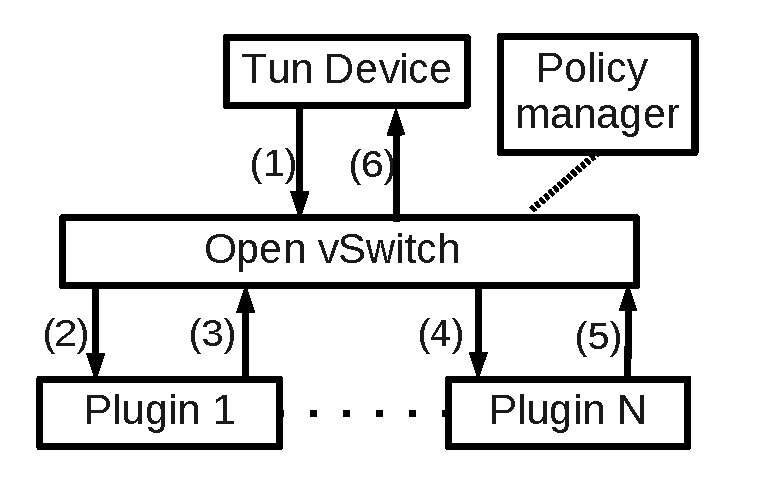
\includegraphics[width=0.8\columnwidth]{figures/packet-monitoring-plugin.pdf}
\end{center}
\caption{Plugin Infrastructure on \platname.}
\label{fig:packet-monitoring-solution}
\end{figure}

A key limitation of previous approaches to measuring mobile 
network traffic is that the contents of encrypted (SSL) traffic 
are unavailable for analysis. Of course, SSL rightfully provides 
authentication and protects user privacy from eavesdroppers; 
however, as increasing amounts of Web traffic flow over HTTPS, 
we lose the ability to understand how to optimize such traffic. 
This has implications both for performance (page speed optimizations) 
and privacy (PII leakage over secure channels). In this section, 
we describe how \platname{} allows us to analyze the contents 
of SSL flows generated by mobile devices. 

\noindent\textbf{Plugin infrastructure.} Figure~\ref{fig:packet-monitoring-solution} shows how we use 
our virtual network interface (TUN) to support a plugin
infrastructure for \platname. Each plugin takes as input a 
network flow and outputs a network flow (potentially empty). 
When a packet is received at the TUN
device, it is sent to a software-defined switch~\cite{Openvswitch} that 
determines the ordered set of plugins that flows will traverse. 
This order is configured by a policy manager, which determines 
the set of plugins that should operate on each flow. After the last 
plugin is traversed, the network flow is sent out through the TUN device 
to the Internet. 

Plugins can be used for many different purposes such as ad blocking, 
analyzing PII leakage or page speed optimization. In the following, we 
describe how we use a plugin to enable SSL traffic decryption using 
the \platname{} plugininfrastructure. 


\noindent\textbf{Example plugin: SSL bumping.} 
First, we note that our VPN proxy implementation uses a self-generated 
\platname{} root certificate that is used to sign all subsequent certificates 
issued to participating mobile devices. This allows us to perform SSL 
traffic decryption, using the Squid proxy's SSL bumping\tbd{AR: give a 
reference} feature, which is essentially a man-in-the-middle operation 
on the secure connection.\footnote{Note that for privacy reasons we do not 
decrypt traffic generated by human subjects; rather, we use this for controlled 
experiments in the lab setting.} Specifically, when the mobile device connects 
to a service supporting SSL, the proxy impersonates the service using a forged certificate signed
with the root certificate of the \platname{} platform. Then the proxy
establishes an SSL connection with the intended target, impersonating a mobile
device. Using the traffic dumped by the tcpdump process as shown in
Figures~\ref{fig:packet-monitor-c} and \ref{fig:packet-monitor-d}, and
using the private key generated by the squid proxy to communicate with
the mobile device, we can decrypt all SSL traffic. We note that when
traffic is not encrypted using SSL, the proxy simply acts as a
transparent proxy. 

This approach will fail for any app that does not trust certificates 
signed by anything other than a well known root authority. 
Surprisingly, this is rarely the case. Whereas the
Twitter application and the Firefox browser prevent SSL bumping by
validating the root certificate, Google Chrome, Safari, the Facebook
application, the Google+ application, the default mail clients, and
advertisement services do not check the validity of the root
certificate. This enables our approach to provide visibility into 
secure channels established the a wide range of popular apps. We will discuss
further this issue in Section~\ref{sec:classification}. 

% \begin{figure}
% \begin{center}
% \includegraphics[width=0.8\columnwidth]{figures/tun-device.pdf}
% \end{center}
% \caption{Tun-tap device to loop packets for packet monitoring.}
% \label{fig:packet-monitoring-solution}
% \end{figure}

% To monitor the packets that are encapsulated within IPsec packets we
% route the packets through a tun-tap device before encryption and after
% decryption.  As shown in \fref{fig:packet-monitoring-solution},

% \subsubsection{Transparent Proxy}
% \label{sec:platform-transparent-proxy}


\subsection{Limitations and Deployability}
\label{sec:addit-limit}

\platname{} provides a scalable way to achieve pervasive, portable 
and passive monitoring of network traffic from mobile devices. In 
this section, we discuss several issues that impact the coverage 
and deployability of our approach. Note that these limitations have 
not significantly impacted our ability to measure mobile networking 
traffic or to deploy our approach to users.

\subsubsection{Limitations}

\drc{Add text about monitoring only one interface.}

\noindent\textbf{At most one tunnel.} Currently iOS and Android 
support exactly one VPN connection at a time. This allows \platname{} 
to measure traffic over either WiFi or cellular interfaces, but not both at once. 
The vast majority of traffic uses only one of these interfaces, 
and that interface uses the VPN.

\noindent\textbf{Proxy location.} All traffic is proxied through a \platname{} box, thus the Web
services will see the \platname{} box address as the end-point and not
the mobile device. This might have an impact in case of Web service
tailoring the answer according to the IP address of the mobile device
(e.g., in case of localization). The biggest problem is when a Web
service deny access to some geographic area, but this problem can be
worked around by installing a \platname{} box on a local (to the Web
sevice) machine.

\noindent\textbf{ISP support.} Some ISPs block VPN traffic. In that case it is not possible
to use the \platname{} platform from a mobile device connected to
such an ISP. There are few ISPs blocking VPN traffic, and there is a
strong incentive to enable VPN traffic in order to attract
professional clients. 

\noindent\textbf{Limited ISP characterization.} \platname{} cannot detect traffic 
differentiation or any other techniques that ISPs use to interpose on network 
traffic using deep packet inspection (such as
advertisement insertion \tbd{AR: give a reference}) or optimization
(such as traffic compression \tbd{AR: give a reference}). This is because the traffic between mobile devices and \platname{}
is encrypted.

\noindent\textbf{IPv6.} \platname{} cannot be currently used on networks using IPv6
because IPv6 is not fully supported by mobile devices. Indeed, we
observe that though iOS and Android support IPv6 they currently do not
support IPv6 traffic through VPN tunnels.

\tbd{Should we use the tripewire experiment? Currently the description
looks like a very small contribution, and it does not bring much to
the discussion. }

\subsubsection{Deployability}
\platname{} uses standard and often open-source software to 
manage and record traffic from mobile devices, making it easy 
to deploy to users and servers. However, a key question is whether 
the system is sufficiently efficient to minimize impact on user behavior 
for our studies in the wild. We show empirically the the overheads are 
reasonable, and provide a brief discussion of incentives for users to 
adopt our system.

We identify the following key aspects of user-perceived inefficiency from 
proxying their network traffic through \platname{}: 
\begin{itemize}
\item \textbf{Establishment delay.} We made a simple set of 50 VPN establishments on both iOS (on an
iPhone 5 running iOS 6.1) and Android (on a Galaxy Nexus running
Android 4.2), and for both \wifi{} and cellular connections. For
Android, we found maximum VPN establishment of 0.81 second on \wifi{}
and of 1.59 second on cellular. For iOS that uses the older IKEv1, the
VPN establishment takes longer: we observe a maximum of 2 seconds on
\wifi{} and 2.18 seconds on cellular.  In summary, for most long term
traffic monitoring experiments, the VPN establishment delay is
negligible. \drc{median?}
\item \textbf{Encapsulation overhead -- data consumption.} \platname{} uses IPsec for datagram encryption, thus there is
an encapsulation overhead for each packet exchanged between the mobile
device and the \platname{} box. To evaluate this overhead, we logged
for 30 days and 25 mobile devices the size of all IPsec packets and of
the encapsulated packet. We observe a maximum increase in the packet
size due to the IPsec encapsulation of 12.8\%. Within the scope of the
traffic monitoring experiments performed with \platname{}, the impact
of this overhead is negligible. However, in case of experiments with a
limited cellular data plan, this overhead must be taken into account.

\item \textbf{Encapsulation overhead -- power consumption.}
To establish and maintain a VPN tunnel, the mobile devices need
additional resources that translate into a larger battery drain during
experiments. To evaluate this battery consumption due to the VPN, we
used a power meter to measure the draw from a Galaxy Nexus running
Android 4.2. We run 10-minute experiments with and without the VPN
enabled. For each experiment, we generated an intensive activity such
as Web searches, map searches, Facebook interaction, e-mail and video
streaming. We found that the VPN leads to a 10\% power overhead. 

We used a power meter on an Android device only because power
measurements require physical access to the battery for a device,
which is not feasible for iOS devices. For iOS devices we conducted
an experiment using video streaming to drain a fully charged battery with 
and without the VPN enabled. We again found approximately 10\% power overhead. 

In summary, the power overhead is low enough to run long experiments
using mobile devices on \platname. To further reduce this overhead (which 
is primarily for cryptographic operations), we are investigating using NULL 
encryption (\ie no encryption) for users that do not need 
the additional privacy enabled by our VPN proxy.

\end{itemize}

\noindent\textbf{Incentives.} We have developed a variety of user incentives that can offset the costs of 
\platname{}; here, we name a few of the most interesting ones.\footnote{We have implemented most of these examples, 
but their details are beyond the scope of this paper.} For example, 
we can provide users with fine-grained views of privacy leaks from 
their applications, and allow them to enable a \platname{} plugin that 
blocks PII. In addition, we are investigating the opportunities for page 
speed optimization. Last, we have implemented opt-in device-wide ad-blocking, 
which can reduce the volume of costly cellular traffic transferred by a device. 


%
%
%VPN establishment delay,
%data consumption overhead due to the VPN encapsulation, power
%consumption overhead on the mobile device. Then we discuss additional
%limitations such as the one due to the encryption of all the traffic
%between the mobile device and the \platname{} box, encryption
%preventing the access ISP to perform traffic modification and
%optimization. 
%% Finally, we discuss the scalability of a single
%% \platname{} box.
%
%\subsubsection{VPN Establishment Delay}
%To establish a VPN tunnel, the mobile device and the \platname{} box
%must negotiate, which takes time. iOS devices use IKEv1 to establish VPN
%tunnels, whereas Android devices use the more recent and faster IKEv2.
%
%% The iOS devices use IKEv1 to manage the VPN tunnels while Android
%% devices support both IKEv1 and IKEv2.  To establish the VPN tunnel,
%% IKEv1 requires a total of 16 packets to be exchanged between the
%% mobile client and the VPN server while IKEv2 requires 4 packets.
%% \platname uses IKEv2 for Android devices while IKEv1 is used for iOS
%% devices.
%
%We made a simple set of 50 VPN establishments on both iOS (on an
%iPhone 5 running iOS 6.1) and Android (on a Galaxy Nexus running
%Android 4.2), and for both \wifi{} and cellular connections. For
%Android, we found maximum VPN establishment of 0.81 second on \wifi{}
%and of 1.59 second on cellular. For iOS that uses the older IKEv1, the
%VPN establishment takes longer: we observe a maximum of 2 seconds on
%\wifi{} and 2.18 seconds on cellular.  In summary, for most long term
%traffic monitoring experiments, the VPN establishment delay is
%negligible. \drc{median?}
%
%% To measure the time required to establish a VPN tunnel, we performed
%% controlled tests using one Android device and an iPhone 5.  We
%% performed these tests from two different locations based in the same
%% city in which the server was deployed.  OUr tests involved
%% \tbdv{number} of VPN tunnel creation over a time period of \tbdv{}
%% hours.  When the Android device used \wifi to establish the VPN
%% tunnel, we observe a median connection establishment time of 0.62
%% seconds from both locations with a maximum of 0.81 seconds and 0.79
%% seconds respectively.  When the Android device used cellular networks
%% to establish the tunnel, the median connection establishment time was
%% 0.81 seconds from both locations with a maximum of 1.59 seconds.
%
%% Compared to the Android device, the iOS devices required a larger
%% amount of time to establish the connection because it relies on a an
%% older key authentication protocol.  From the two Wi-Fi networks, to
%% establish the VPN tunnel, the iOS device required 1.60 seconds and
%% 1.34 seconds with a maximum of 2.0 seconds and 1.48 seconds
%% respectively; in the case of cellular networks we observed a median of
%% 1.80 seconds and 1.65 seconds with a maximum of 2.18 seconds and 1.87
%% seconds respectively. \drc{This needs to go in a table, since it is
%%   impossibly dense.}
%
%% \tbd{In summary, we observe that because iOS devices use an older key
%%   exchange protocol they can take up to twice as much time as Android
%%   devices to establish the VPN tunnel.  Any more insights .. The
%%   tunnel establishment times in the order of 2 seconds implies that
%%   \platname can have a significant latency overhead if VPN tunnels are
%%   established periodically for short tests.}
%
%\subsubsection{Data Consumption Overhead}
%\platname{} uses IPsec for datagram encryption, thus there is
%an encapsulation overhead for each packet exchanged between the mobile
%device and the \platname{} box. To evaluate this overhead, we logged
%for 30 days and 25 mobile devices the size of all IPsec packets and of
%the encapsulated packet. We observe a maximum increase in the packet
%size due to the IPsec encapsulation of 12.8\%. Within the scope of the
%traffic monitoring experiments performed with \platname{}, the impact
%of this overhead is negligible. However, in case of experiments with a
%limited cellular data plan, this overhead must be taken into account. 
%
%
%% IPSec encapsulation slightly inflates packet sizes, in addition to
%% preventing carrier middleboxes from applying their own compression.
%% We measured the overhead of the tunnel in terms of data overhead from
%% IPsec headers and keep-alive messages, finding that it ranges from
%% 8--12.8\%.
%
%% To compute the increase in the amount of bytes transferred due to
%% encapsulation and the keep-alive messages, we log the packet lengths
%% of the encrypted packets (IPsec packets) exchanged by our \platname
%% servers and the mobile clients.  We performed this packet capture for
%% 30 days during which 25 devices tunneled their traffic via \platname.
%% During this time interval we also log the packet length of the packets
%% encapsulated within the IPsec packets.  During this 30 day period we
%% observe that the median of the increase to be 8.31\%, with a maximum
%% increase of 12.8\%.
%
%% \tbd{In summary, we observe a maximum overhead of 12.8\% increase in data consumption. We believe the costs of this overhead are minimal compared to the cost of warrant voiding the device.}
%
%\subsubsection{Power Consumption Overhead}
%To establish and maintain a VPN tunnel, the mobile devices need
%additional resources that translate into a larger battery drain during
%experiments. To evaluate this battery consumption due to the VPN, we
%used a power meter to measure the draw from a Galaxy Nexus running
%Android 4.2. We run 10 minutes experiments with and without the VPN
%enabled. For each experiment, we generated an intensive activity such
%as Web searches, map searches, Facebook interaction, e-mail and video
%streaming. We found that the VPN leads to a 10\% power overhead. 
%
%We used a power meter on an Android device only because power
%measurements require physical access to the battery for a device,
%which is not feasible for iOS devices. For iOS devices we made
%simpler experiments consisting in draining a fully charged battery with
%a video streaming with a without the VPN enabled. We found also around
%a 10\% power overhead. 
%
%In summary, the power overhead is low enough to run long experiments
%using mobile devices on \platname. 
%
%% \footnote{We use Android because power measurements
%%   require physical access to the battery for a device, which is not
%%   feasible for iOS devices. We found similar results when testing the
%%   time to discharge an iOS device while streaming video with and
%%   without a VPN connection.}
%
%% We found that VPN proxying imposes approximately 10\% power overhead
%% compared to direct traffic. To test the additional power consumption
%% from using a VPN proxy, we used a power meter to measure the draw from
%% a Galaxy Nexus running Android 4.2.\footnote{We use Android because
%%   power measurements require physical access to the battery for a
%%   device, which is not feasible for iOS devices. We found similar
%%   results when testing the time to discharge an iOS device while
%%   streaming video with and without a VPN connection.} While
%% instrumented, we conducted 10-minute experiments where we scripted
%% device usage with and without a VPN enabled. The activities included
%% Web searches, map searches, Facebook interaction, e-mail and video
%% streaming.
%
%\subsubsection{Additional Limitations}
%

% To understand whether traffic interposition by ISPs is frequent, we
% made a dedicated experiment using tripewires\tbd{cite the paper}.  In
% particular, we exploit Android's support for apps providing VPN
% services; instead of establishing a secure connection we simply
% forward traffic to a proxy server without additional encryption. In
% this way, the mobile device's ISP can inspect the contents of all
% non-SSL traffic and interpose accordingly.  Note that one limitation
% of this approach is that the ISP will see the destination for all
% network traffic is our proxy server (instead of the original
% destination), which could impact how ISPs treat the corresponding
% traffic.

% T-Mobile  AT&T 1000 first alexa rank, in France Orange and Free. 

% VPN proxying via secure tunnels prevent ISPs from inspecting or
% interposing on network traffic, thus preventing us from measuring this
% behavior. To understand ISP interference with mobile Internet traffic,
% we additionally support measurement using an \emph{insecure}
% transparent proxy.  In particular, we exploit Android's support for
% apps providing VPN services; instead of establishing a secure
% connection we simply forward traffic to a proxy server without
% additional encryption. In this way, the mobile device's ISP can
% inspect the contents of all non-SSL traffic and interpose accordingly.
% Note that one limitation of this approach is that the ISP will see the
% destination for all network traffic is our proxy server (instead of
% the original destination), which could impact how ISPs treat the
% corresponding traffic.


% \tbd{In summary, despite these shortcoming we believe that \platname can be used for realistic measurements of mobile Internet traffic.}




%%% Local Variables: 
%%% mode: latex
%%% TeX-master: "main.tex"
%%% End: 
